\begin{figure}[t!]
\centering
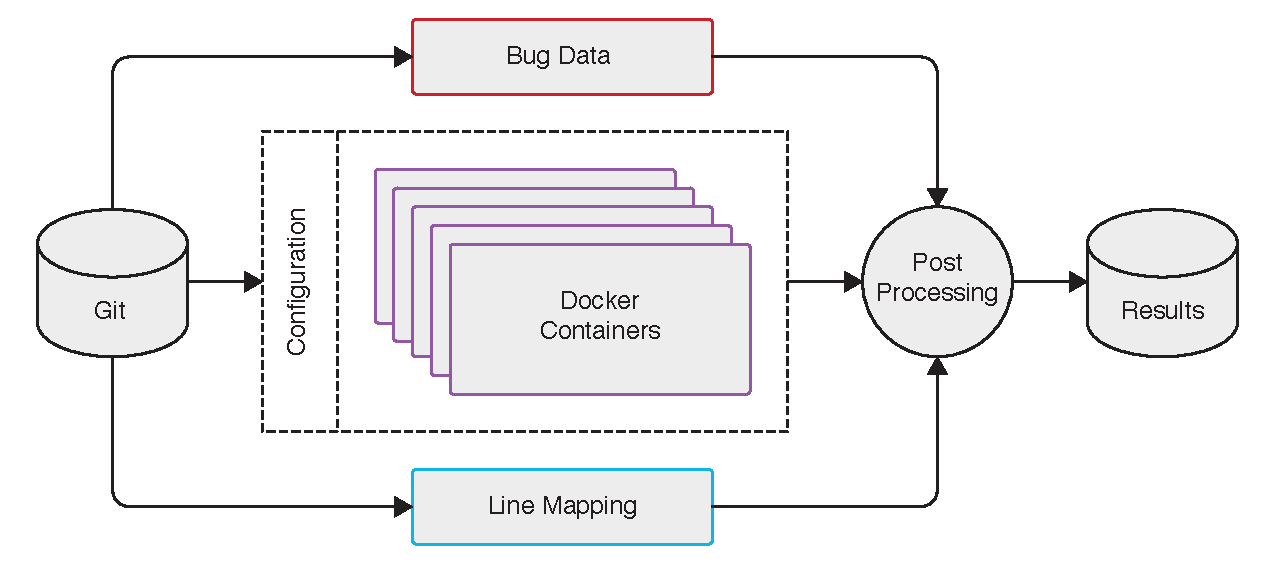
\includegraphics[width=\columnwidth]{evolution/figures/pipeline}
\caption{\covrig infrastructure.}
\label{fig:arch}
\end{figure}

The overall architecture of the \covrig infrastructure is depicted
in Figure~\ref{fig:arch}.  It contains a generic driver which
iterates through all the revisions in a given range and invokes
routines specific to each system to compile, run, and collect
statistics of interest.

%% To collect information about each program revision, such as whether it
%% successfully compiles, whether it passes the regression tests and with
%% what coverage, we built an infrastructure capable of automatically
%% retrieving and compiling each version of a target program, running
%% existing regression tests and collecting metrics of interest.

%The system is built on top of software containers~\cite{}, a
%lightweight virtualisation mechanism, which offers both isolation and
%reproducibility, by ensuring a consistent environment into which to
%run each software revision.  In this way, the execution of different
%revisions do not influence each other, \eg by inadvertently leaving
%behind lock files or not properly freeing up resources.

\paragraph{Lightweight software containers} \covrig employs software
containers~\cite{containers:eurosys07}, an operating system-level
virtualisation mechanism that provides the ability to run multiple
isolated virtual Linux systems (``containers'') inside a single host
OS.  When launched, \covrig starts by loading the selected range of
revisions from the project's \git repository, and for each revision
starts a new software container.  The use of containers offers
increased isolation and reproducibility guarantees by providing a
consistent environment in which to run each software revision and
ensuring that different revisions do not interfere with each other,
\eg by inadvertently leaving behind lock files or not properly freeing
up resources.

The choice of lightweight OS-level virtualisation rather than more
traditional virtual machines (\eg
\kvm\footnote{\url{http://www.linux-kvm.org/}} or
\xen\footnote{\url{http://www.xenproject.org/}}) reduces the
performance penalty associated with spawning and tearing down VMs,
operations performed for each revision analysed.  To get a sense of
this difference, we compared an
\lxc\footnote{\url{http://linuxcontainers.org/}} container, which
required under a second for these operations, with a \xen VM, which
needed over a minute.

In our implementation, we use
\docker\footnote{\url{https://www.docker.io/}} to create and manage
the lower-level \lxc containers, and
%Vagrant to
deploy them on multiple local or cloud machines.
Each container is used to configure, compile and test one
program revision, as well as collect the metrics of interest, such as
code size and coverage. The containers are remotely controlled through
SSH using the \fabric\footnote{\url{http://fabfile.org/}} framework.


\paragraph{Configuration file} \covrig has a modular architecture, which makes it
possible to analyse new systems with modest effort. A potential user
of our infrastructure only needs to provide a Python
configuration file describing the system.  A minimal file provides
the name of the system, its \git repository location, a method to
compile the system, \eg install dependencies and run the appropriate
\stt{make} command, and a method to run the regression tests, \eg run
the \stt{make test} command.
%
Finally, the configuration file can also specify an {\em end revision}
and a specific number of revisions to analyse.  
%% \covrig will use these parameters to determine the list of revisions to
%% analyse, independent of the target system's evolution.  
For accurate test suite size measurements, the files or folders which
make up the test suite can also be indicated.

For each revision, \covrig collects several static and dynamic metrics.  The
static metrics are obtained either directly from the version control
system (\eg the number of lines of test code) or after compiling each
revision (\eg the number of executable lines of code).  The dynamic
metrics require running the regression tests (\eg the overall line
coverage or the regression test success status).

Further information and graphs---including the ones presented in our
empirical study---are automatically derived in the post-processing
stage from these primary metrics using a set of scripts.

%% For example, we were able to verify that the {\em latent patch
%% coverage}, \ie the fraction of code which is executed only several
%% revisions after it is introduced is small, and practitioners can
%% safely ignore it most of the time when evaluating test suite
%% augmentation or coverage-improvement techniques.


%\subsection{Bug Data} \label{ssec:bugdesign}

\paragraph{Bug data} One possible application of \covrig is finding
useful data about software bugs and correlating them with the static
and dynamic metrics collected. For our study, we mined bug data from
both software repositories and, where available, bug tracking systems.
We automatically obtained a list of candidate bug-fixing revisions by
iterating through the list of commits and checking the commit message
for words such as {\em fix}, {\em bug} or {\em issue}, followed by a
number representing the bug identifier.  For example, a typical
\memcached bug fix commit message looks like {\em "Issue 224 - check
  retval of main event loop"}. The regular expression that we used to
identify these commits is similar to the ones used in prior
work~\cite{genealogies:issre13}:

\lstinline`(?:bug|issue|fix|resolve|close)\s*\#?\s?(\d+)`

Where possible, we confirmed that the bug identifier is valid by
querying the associated bug tracking system. We further manually
checked all reported revisions and confirmed that they included no
false positives.  While it is impossible to quantify the false
negative rate without a knowledgeable developer manually checking all
the revisions in a repository, we believe that the automatically
obtained bug fixes create a representative subset of the fixes in the
repository.

\paragraph{Line mapping} The ability to track how lines move and change
across revisions is the cornerstone of many high-level software
evolution analyses.  A line mapping algorithm improves over the
traditional \diff algorithm by tracking the movement of individual
lines rather than hunks.  Conceptually, line mapping is a function
which takes two revisions, \textit{r1} and \textit{r2}, and a program
location described by a pair \textit{(file name 1, line number 1)}
associated with \textit{r1}.  The output is a pair \textit{(file name
  2, line number 2)} identifying the corresponding location in
\textit{r2}.

Our implementation of the line mapping algorithm is similar to the
algorithms described in previous
work~\cite{szz:msr05,szz:ase06,change-source-code:msr07,szzrevisited:defects08}.
It makes use of the \emph{Levenshtein edit
  distance}~\cite{levenshtein1966binary} to track line edits, and
\emph{tf--idf}~\cite{tf-idf} and \emph{cosine
  similarity}~\cite{cosinesimilarity} to track line movements.  It
also uses the \emph{Hungarian algorithm}~\cite{hungarian} to find the
optimal matching of lines across versions.  Compared to previous work,
our implementation can also improve precision by using coverage information to filter
non-executable lines.

%% We used line mapping in two ways in our analysis: to determine whether
%% patches are tested within the next few revisions after they were
%% created (\S\ref{sec:lpcoverage}), and to estimate where bugs were
%% introduced (\S\ref{sec:bugs}).

In our study, we used line mapping to determine whether patches are
tested within the next few revisions after they were created
(\S\ref{sec:lpcoverage}).

\paragraph{Cloud deployment} To enable large-scale data collection and
processing, we deployed \covrig to our private cloud.  We have built our
system around a standard set of tools: Packer for building custom
Docker-enabled machine images, Vagrant for controlling and provisioning
the virtual machines based on these images, a Docker registry for
serving \covrig's Docker containers and a {\em fabfile} for
orchestrating the entire cluster. The same set of tools and scripts
can be used to deploy \covrig to different private or public clouds.

%% \subsection{High-Level Questions} \label{ssec:highlevel}

%% Coverage, bugs and line mapping data already provide useful insights into a
%% software project. For example, coverage and known bugs count can be used to
%% predict the residual bugs, i.e., the bugs still present in the software, using
%% a simple formula~\cite{coveragedefects98}

%% Using the bug data, we can quantify the number of patches which attempt to fix
%% a bug but either contain an incomplete fix or introduce new bugs. Such patches
%% are identified by looking for bug pairs, one being fixed and the other
%% introduced in the same patch. A high number of buggy fixes points to
%% deficiencies in the software development process.

%% \todo{More interesting things that we can do directly with coverage, bugs and
%% line mapping data}

%% However, further processing of this data allows us to answer more questions.
%% Combining  bug data and coverage data allows us to determine how many bugs are
%% in code which was already tested, i.e. executed without triggering the bug.
%% This may happen because the bug is only activated in corner-case scenarios.
%% Systems with a high number of bugs present in tested code may benefit from
%% symbolic execution-based testing tools such as ZESTI~\cite{zesti}, which
%% transparently instrument the existing tests to check for corner-case scenarios.
%% On the other hand, systems where the bugs are present in untested code can
%% benefit from test generation tools such as KATCH~\cite{katch}.

%% Correlations between bug data and software metrics can be used to build a bug
%% predictors based on project history and current patch coverage. Integrated in a
%% development environment or continuous integration system, such predictors can
%% warn developers when making high-risk changes. An intuitive predictor is based
%% on patch coverage: a tested patch is less likely to be buggy, compared to an
%% untested patch and the correlation can be mined from the project history. Code
%% churn can also be used as a predictor~\cite{churn-bugs:issre96, churndefects05}
%% and can be further refined to by eliminating non-executable changes or using
%% fine-grained souce code change extraction techniques~\cite{fluri:scc}
%% and its relationship with bugs can be mined using the line mapping data at the
%% line/function/file level.
%% % But we really don't want to go too much into statistics

%% Another question is whether old regression tests are still adequate for the
%% latest program version. We can quantify test adequacy by the fraction of the
%% code originally executed by the test that is still executed in the current
%% version. For an accurate computation we need to map the lines originally
%% executed to their counterparts in the current version.
